\chapter{Evaluation}

In this chapter, we implement FHS and GES into a centralized wireless resource
scheduling problem with underlying GE channel and evaluate the behavior as well
as the performance of our proposed methods in simulations. To provide an
appropriate comparison, in Sec.~(\ref{sec:setup}) we describe our choices for
our simulation environment and introduce three testing scenarios with different
network configurations. Finally, we present and discuss the results of different
simulations in Sec.~(\ref{sec:results}). 

\section{Simulation Setup} \label{sec:setup}
% Details regarding implementation and/or simulation are given in this chapter.
% The considered setup and the parameters used are introduced and discussed. Also,
% the general evaluation methods can be presented. (Note: Code should not be part
% of this chapter. If it makes sense to introduce it into the thesis, it should be
% placed in the appendix.)

Suppose a minimal simulation environment comprising of $N=3$ control
sub-systems sharing a GE wireless channel to demonstrate the benefit of finite
horizon minimization. In order to provide intuitive and illustrative results, we
consider scalar sub-systems in the evaluation. Each sub-system is chosen to have
different plant system dynamics, with increasing unstable system matrices, i.e.,
$A_{1,2,3} = \left\{1.0, 1.25, 1.5\right\}$. The input matrix is given by $B_i =
1.0, \forall i$. The control sub-systems are initialized with $x_i[0] = w_i[0]$
for all $i$ and system noise is characterized by $w_i[k]\sim \mathbb{N}(0,1)$,
i.e., $\Sigma_i=1$. Among the simulated sub-systems, $A_3=1.5$ represents the
most challenging application, as its system state evolves the most absolutely
within a control time step $k$. Moreover, sub-systems are sampled periodically
every 3 slots, i.e., $D_i=3$. To enable non-synchronized sampling, we determine
the initial sampling event randomly from a discrete uniform distribution as
$t_{i,o} = \mathcal{U}\{0, D_i-1\}$. \\
The control law is selected with respect to $\boldsymbol{Q}_i = 1$ and
$\boldsymbol{R}_i = 1$. That is, we solely account for state cost and allow
arbitrary control inputs. According to Eq.~\eqref{eq:optimalgain}, the optimal
feedback gain matrix is determined as $\boldsymbol{L}^*_i = A_i$, which
corresponds to deadbeat control strategy. 

\begin{table}[htb]
  \begin{center}
  \begin{tabular}{|lc|c|c|c|} 
  \hline
  \multicolumn{2}{|c|}{\textbf{Channel model parameters}} & \textbf{Scenario 1} & \textbf{Scenario 2} & \textbf{Scenario 3} \\
  \hline \hline
  Loss in Good & $p_G$ & 0.25 & 0.25 & 0.0011 \\ 
  Loss in Bad & $p_B$ & 0.75 & 0.75 &  0.7734 \\ 
  Failure rate & $f$ & 0.3 & 0.1 & 0.0024 \\ 
  Recovery rate & $r$ & 0.3 & 0.1 & 0.0832 \\
  \hline
  Average error probability & $p_E$ & 0.5 & 0.5 & 0.0227 \\
  Mean sojourn time in Good & $T_G$ & 3.33 & 10 & 416.66 \\
  Mean sojourn time in Bad & $T_B$ & 3.33 & 10 & 12 \\
  \hline
  \end{tabular}
  \end{center}
  \caption{Evaluation scenarios and their Gilbert-Elliot channel parametrization and statistical properties}
  \label{tab:scenarios}
\end{table}

Table~(\ref{tab:scenarios}) depicts the 3 chosen scenarios and their respective
GE channel parametrization, where the channel conditions are getting worse from
set to set. Scenario 1 and 2 resemble balanced GE channels, where on average
half of the packet transmitted are lost. Further, due to symmetrical state
transition probabilities, the channel will be in good and bad states 50\% of the
simulation time each. $f$ and $r$ merely differ in absolute values, making the
second channel prone to longer burst errors. To evaluate scheduler performance
in a real-life scenario, we have adopted the third GE parameters from
experiments conducted in \cite{frohn2011analyzing}. Here, measurements are
obtained from an indoor wireless testbed based on the IEEE 802.11n standard.
Obtained network trace is then used to find analytical GE parameters using the
\textit{Baum-Welch algorithm} \cite{baum1970maximization}. \\ 
For each scenario we vary the finite Horizon $H=\left\{ 1, \cdots, 10\right\}$
for FHS and $H=\left\{ 1, \cdots, 4\right\}$ for GES to study its effect on AoI
and remote estimation performance. Each configuration is simulated for a
duration of $D=20000$ time slots and repeated $R=200$ times.

\subsection{Performance Metrics} 

We evaluate scheduling performance in terms of the following metrics. In every
simulation, the average mean squared error of a sub-system $i$ at each slot is
measured as:

\begin{equation*}
  MSE_i = \dfrac{1}{D} \sum_{t=1}^{D}{(\boldsymbol{e}_i(t))^T \boldsymbol{e}_i(t)},
\end{equation*}

where $\boldsymbol{e}_i(t)$ is the estimation error defined in
Eq.~\eqref{eq:estimationerror}. In addition, we analyze the average MSE in the
network given by:

\begin{equation*}
  \overline{MSE} = \dfrac{1}{N} \sum_{i=1}^{N}{MSE_i}
\end{equation*}

MSE indicates the deviation of the estimated state from its true state, hence,
quantifying estimation accuracy of estimator $\estimator$. In the same fashion,
we measure information freshness at $\estimator$ through measuring average AoI
in the network as follows:

\begin{align*}
  \Delta_i &= \dfrac{1}{D} \sum_{t=1}^{D}{\Delta_i(t)}, \\
  \overline{\Delta} &= \dfrac{1}{N} \sum_{i=1}^{N}{\Delta_i}
\end{align*}

\section{Results and Discussion} \label{sec:results}
% Results of the performed investigations are presented here. Interpretations for
% the observed effects are given and the impact of investigations is discussed. 

\subsection{Remote Estimation Performance}

\begin{figure}[htbp]
  \centering
  \begin{subfigure}[b]{0.49\textwidth}
      \centering
      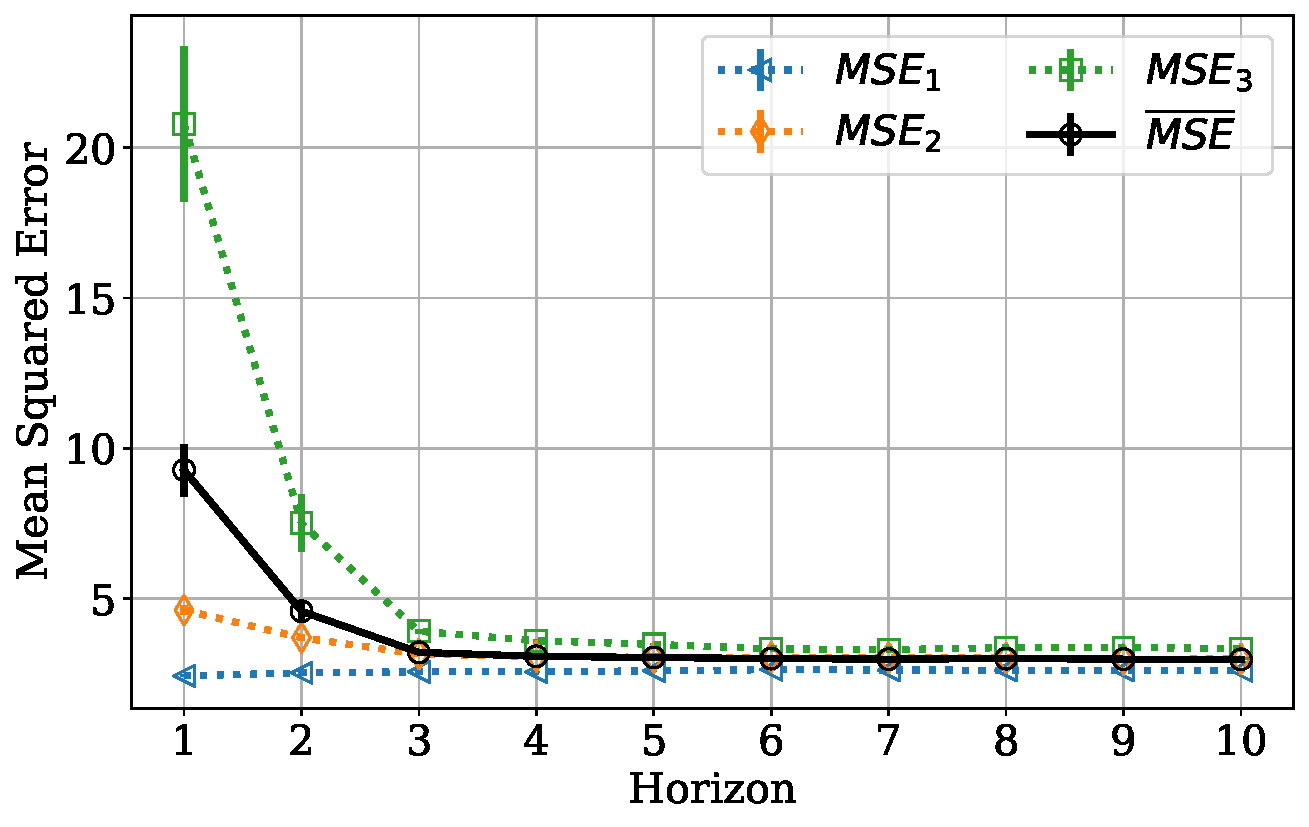
\includegraphics[width=\textwidth]{FHS1_MSE_against_H_separate}
      \caption{Scenario 1 with FHS}
  \end{subfigure}
  \hfill
  \begin{subfigure}[b]{0.49\textwidth}
      \centering
      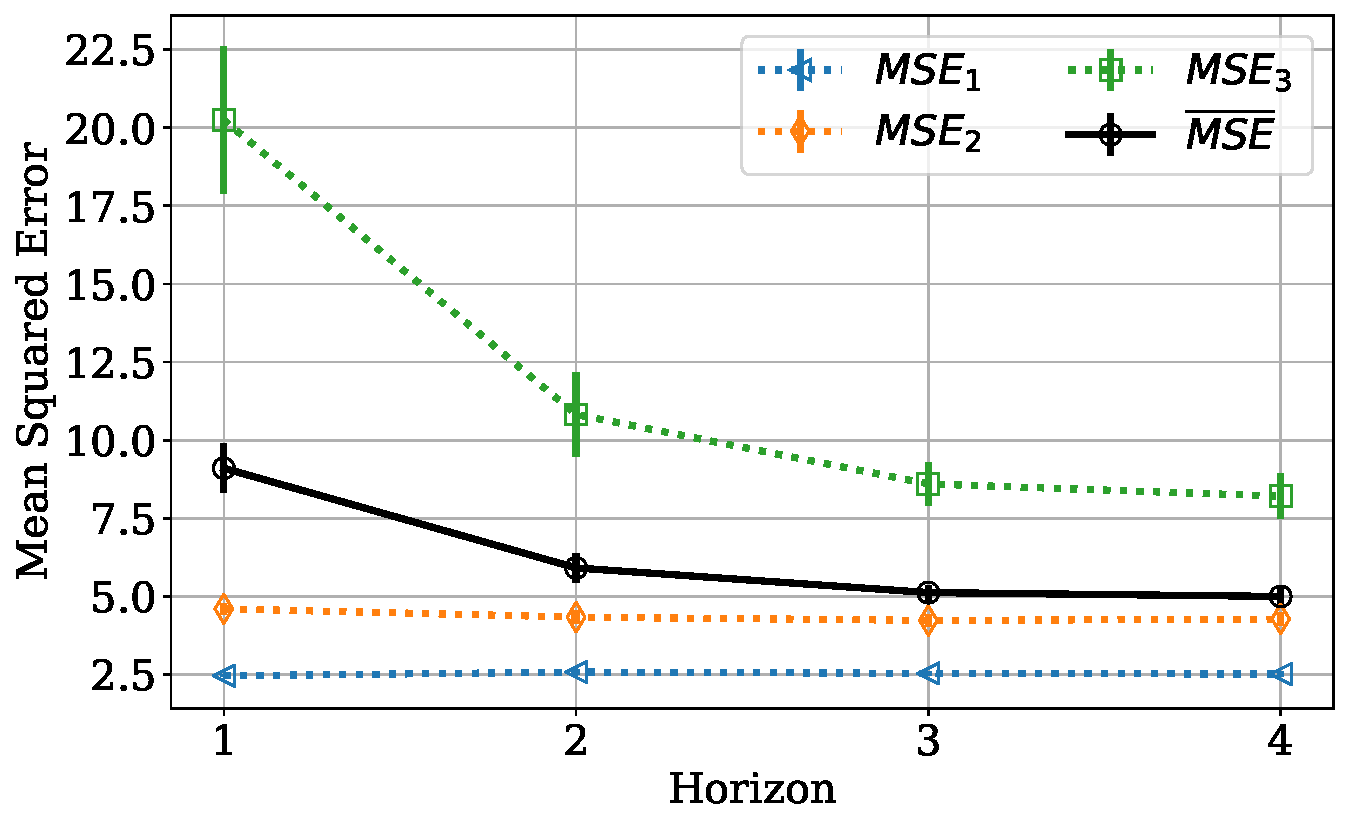
\includegraphics[width=\textwidth]{GES1_MSE_against_H_separate}
      \caption{Scenario 1 with GES}
  \end{subfigure}
     \caption[Scenario 1: Average MSE vs. finite horizon $H$]{Solid line
     $\overline{MSE}$ illustrates the average MSE in the network per time slot.
     Dashed lines $MSE_1$, $MSE_2$ and $MSE_3$ show the the average MSE per time
     slot of each class with $A_1=1.0$, $A_2=1.25$ and $A_3=1.5$, respectively.
     Vertical bars represent $95\%$ confidence interval for $R=200$ simulation
     runs.}
     \label{fig:MSEavg}
\end{figure}

\begin{figure}[htbp]
  \centering
  \begin{subfigure}[b]{0.49\textwidth}
      \centering
      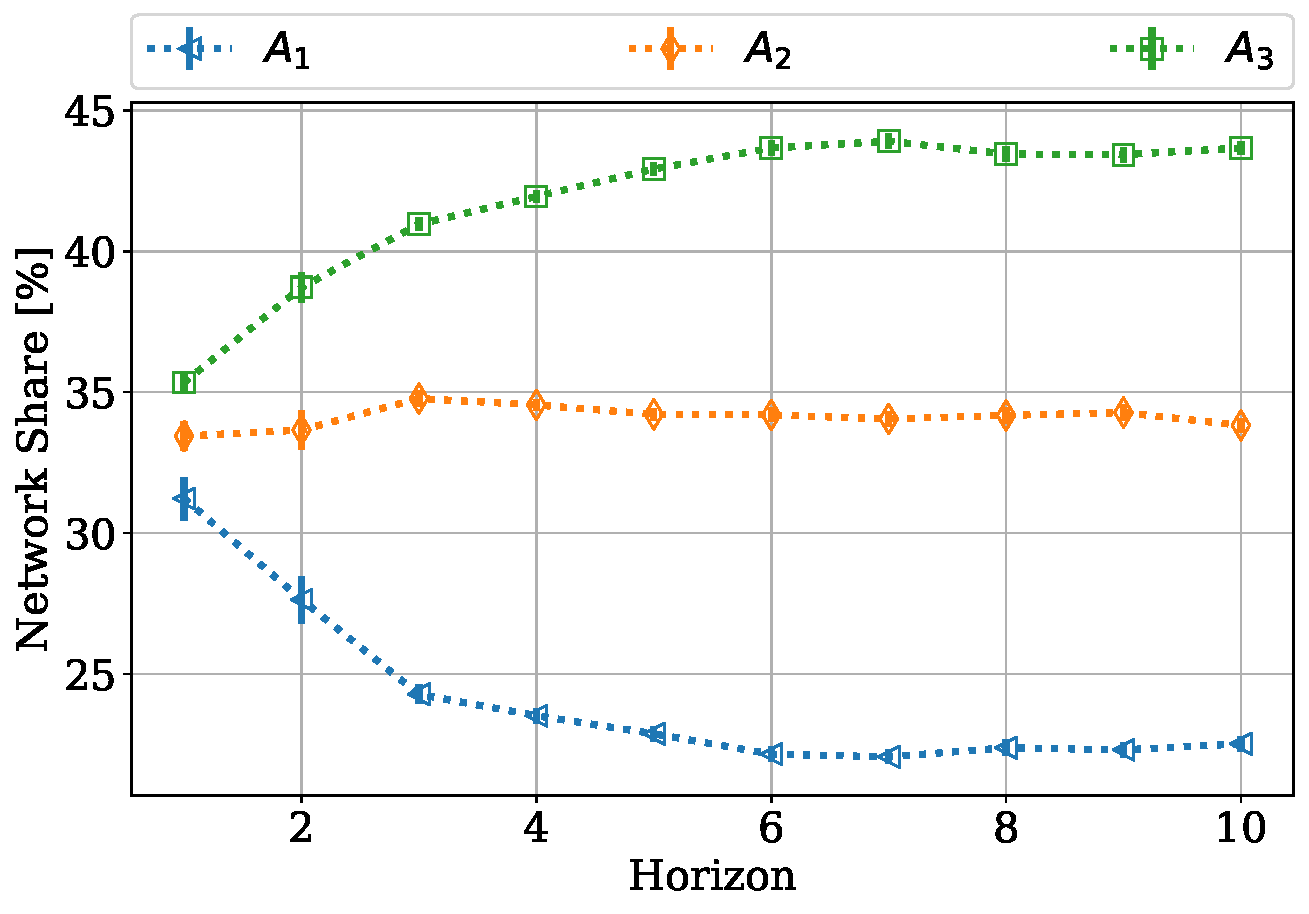
\includegraphics[width=\textwidth]{FHS1_NS_against_H_separate}
      \caption{Scenario 1 with FHS}
  \end{subfigure}
  \hfill
  \begin{subfigure}[b]{0.49\textwidth}
      \centering
      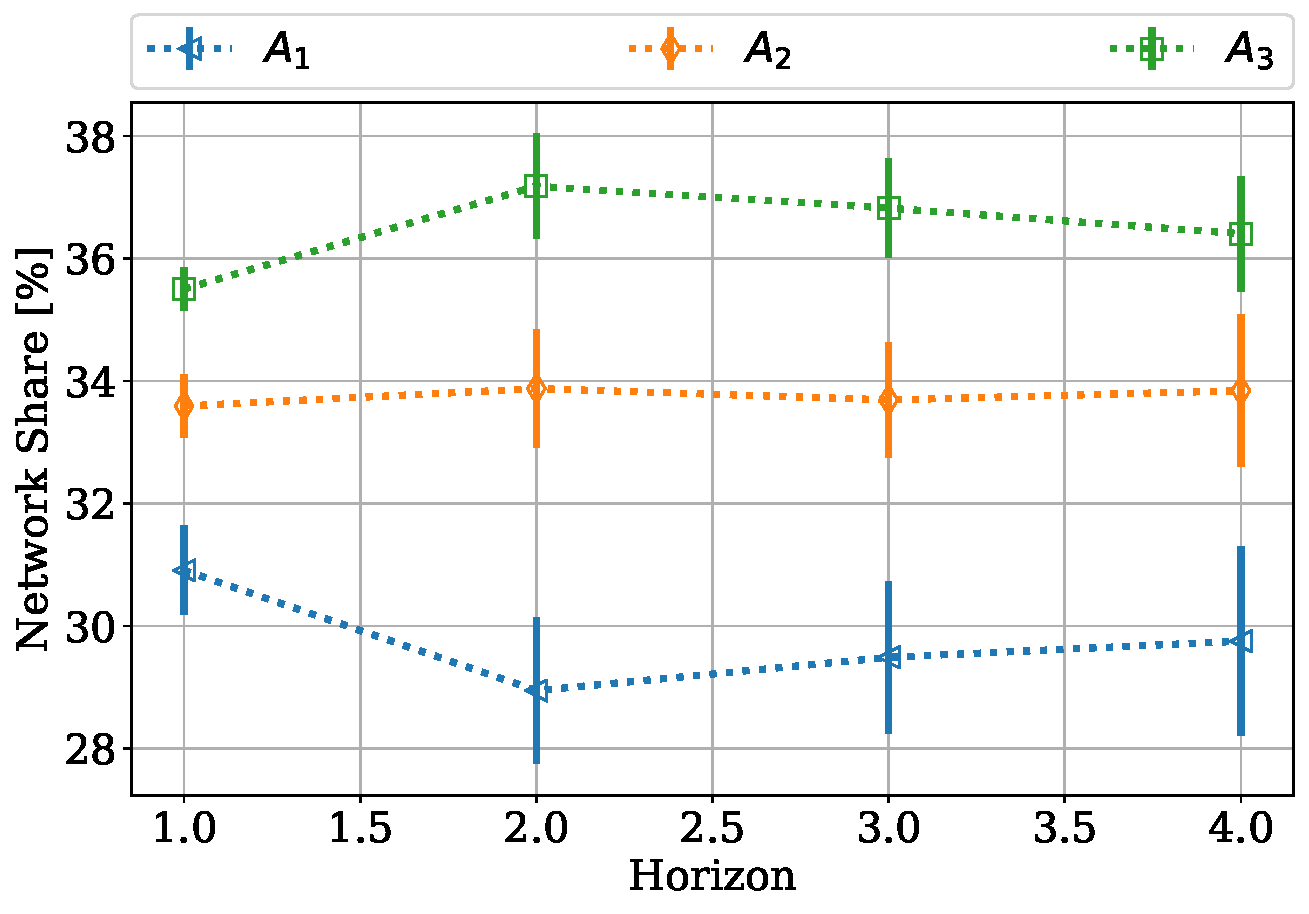
\includegraphics[width=\textwidth]{GES1_NS_against_H_separate}
      \caption{Scenario 1 with GES}
  \end{subfigure}
     \caption[Scenario1: Network resources share among heterogenous subsystems
     vs. finite horizon $H$]{}
     \label{fig:networkshare}
\end{figure}


\subsection{Age-of-Information Performance}

\begin{figure}[htbp]
  \centering
  \begin{subfigure}[b]{0.49\textwidth}
      \centering
      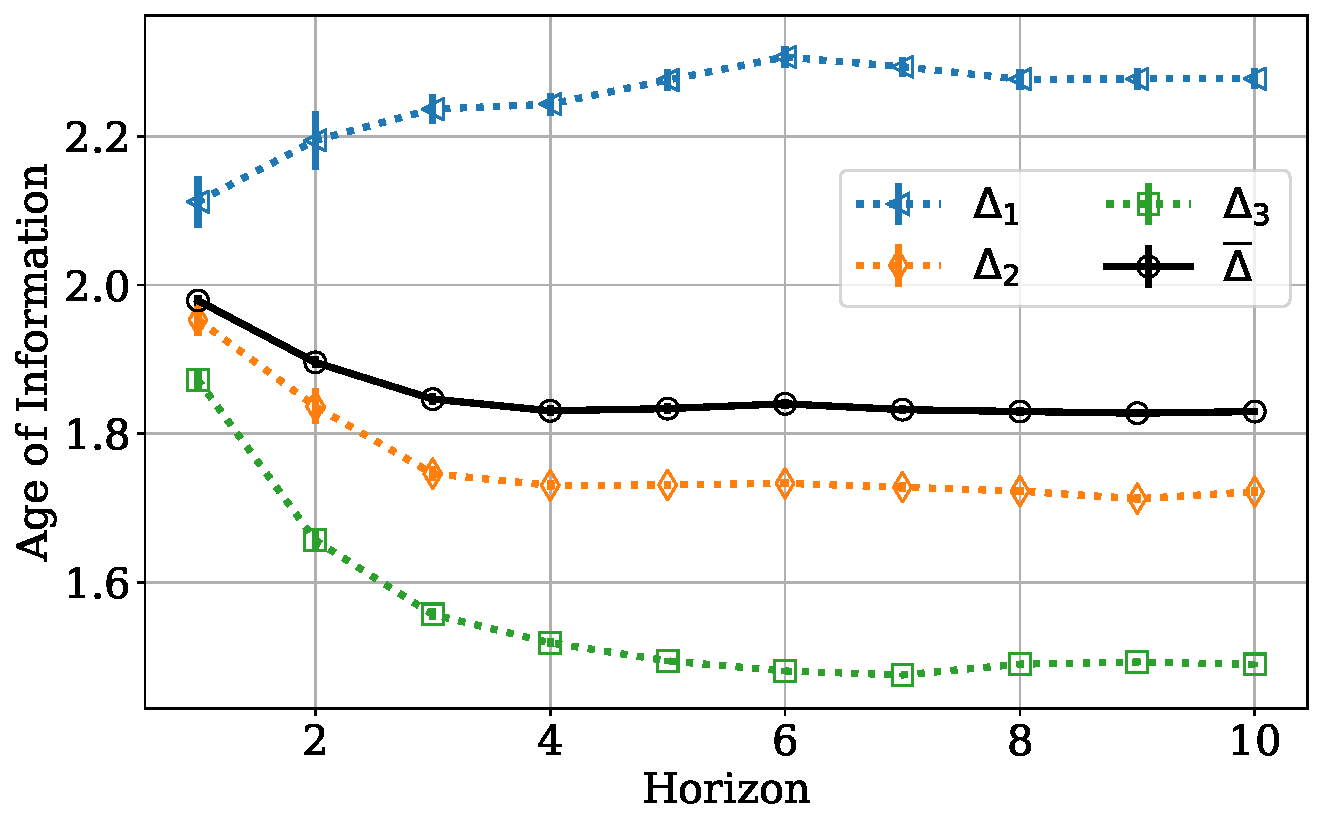
\includegraphics[width=\textwidth]{FHS1_AoI_against_H_separate}
      \caption{Scenario 1 with FHS}
  \end{subfigure}
  \hfill
  \begin{subfigure}[b]{0.49\textwidth}
      \centering
      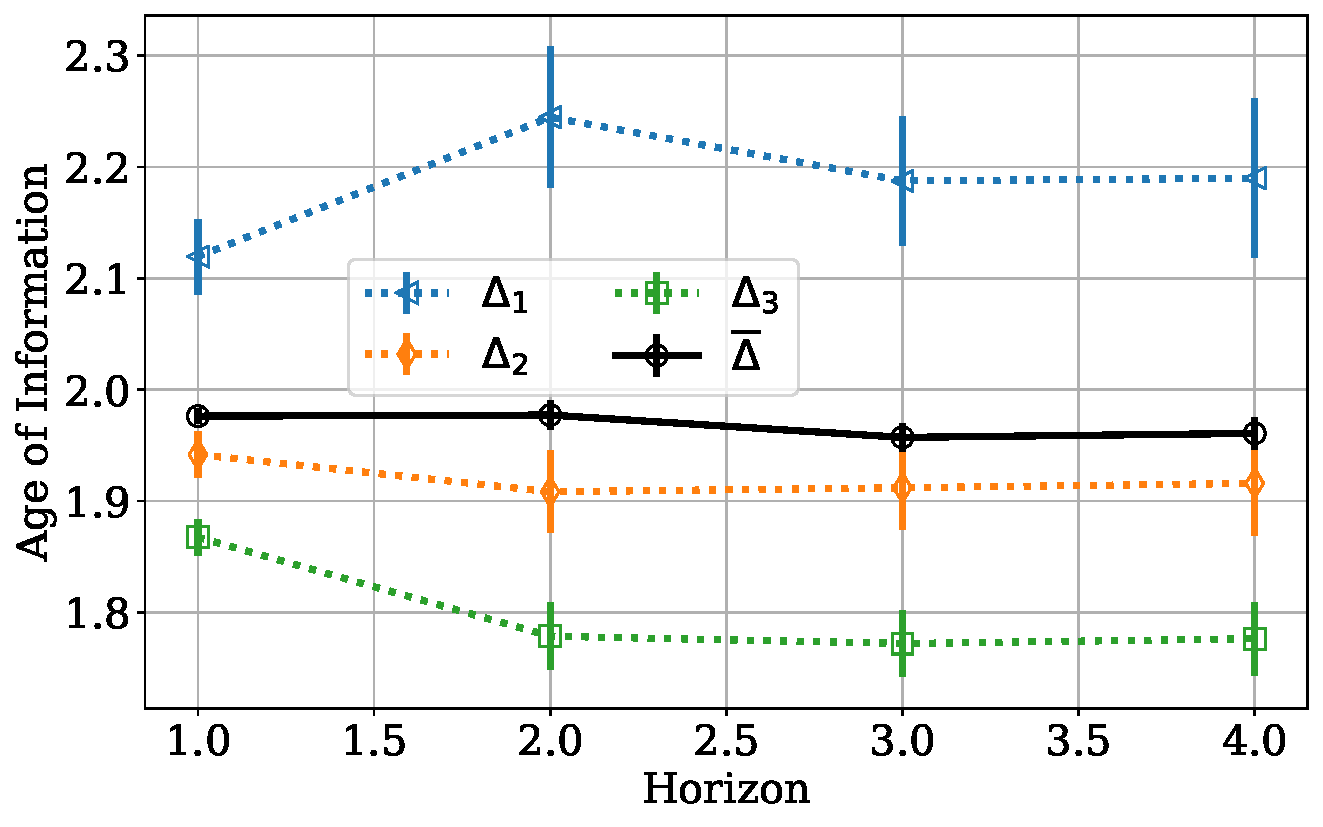
\includegraphics[width=\textwidth]{GES1_AoI_against_H_separate}
      \caption{Scenario 1 with GES}
  \end{subfigure}
     \caption[Scenario 1: Average AoI vs. finite horizon $H$ for Scenario
     1]{Solid line $\overline{\Delta}$ illustrates the average AoI in the
     network per time slot. Dashed lines $\Delta_1$, $\Delta_2$ and $\Delta_3$
     show the the average AoI per time slot of each class with $A_1 = 1.0$,
     $A_2=1.25$ and $A_3=1.5$, respectively. Vertical bars represent $95\%$
     confidence interval for $R=200$ simulation runs.}
     \label{fig:AoIseperate}
\end{figure}

\subsection{Age-of-Information Distribution}

\begin{figure}[htbp]
  \centering
  \begin{subfigure}[b]{0.49\textwidth}
      \centering
      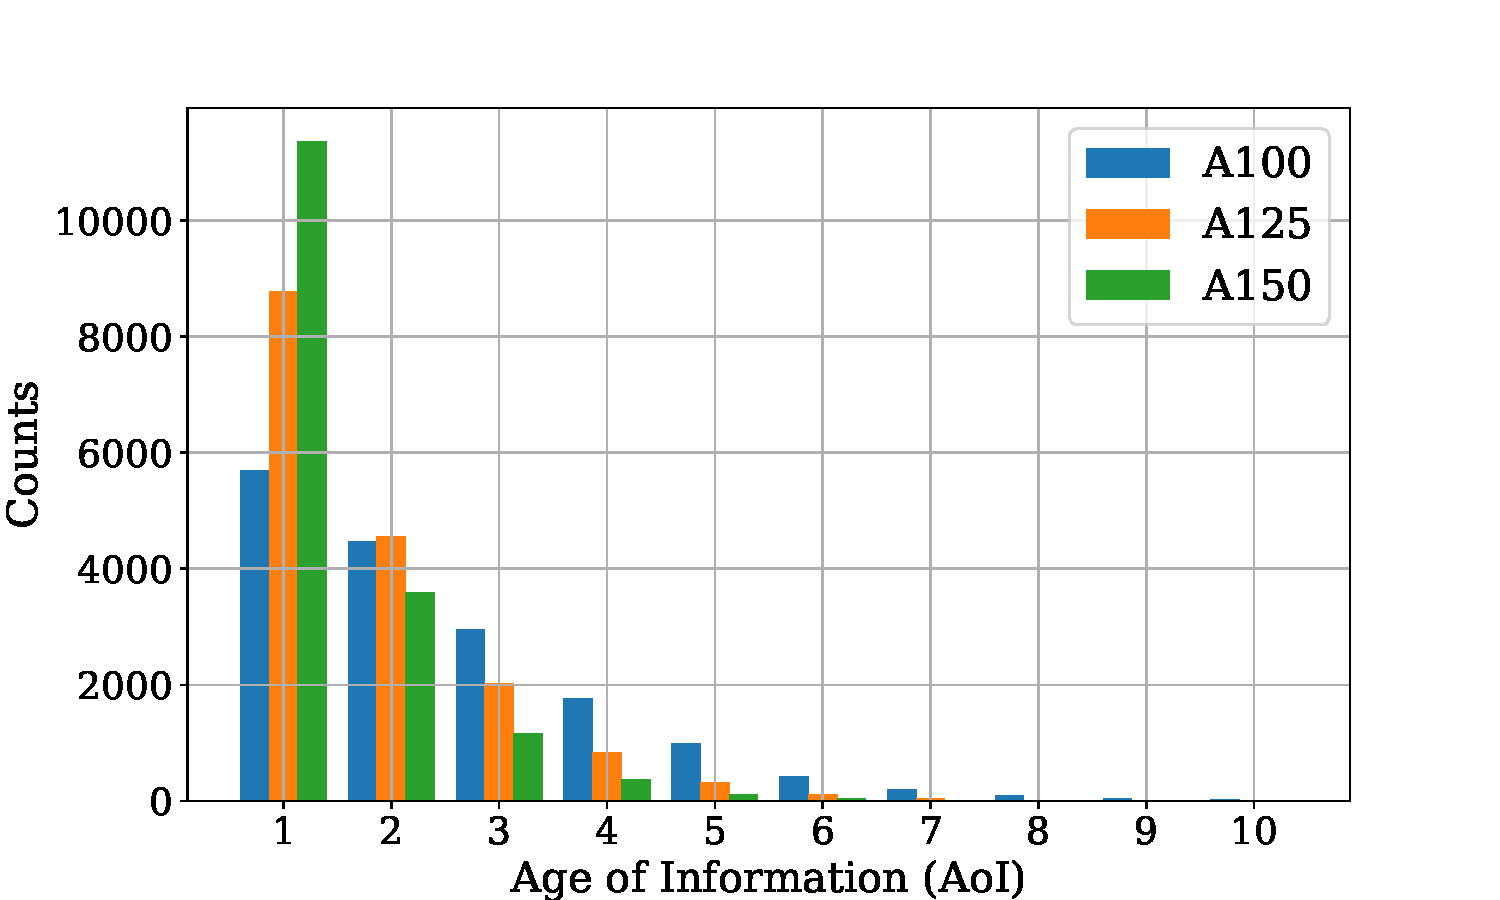
\includegraphics[width=\textwidth]{AoI_Histogram_N3}
      \caption{Scenario 1 with FHS}
  \end{subfigure}
  \hfill
  \begin{subfigure}[b]{0.49\textwidth}
      \centering
      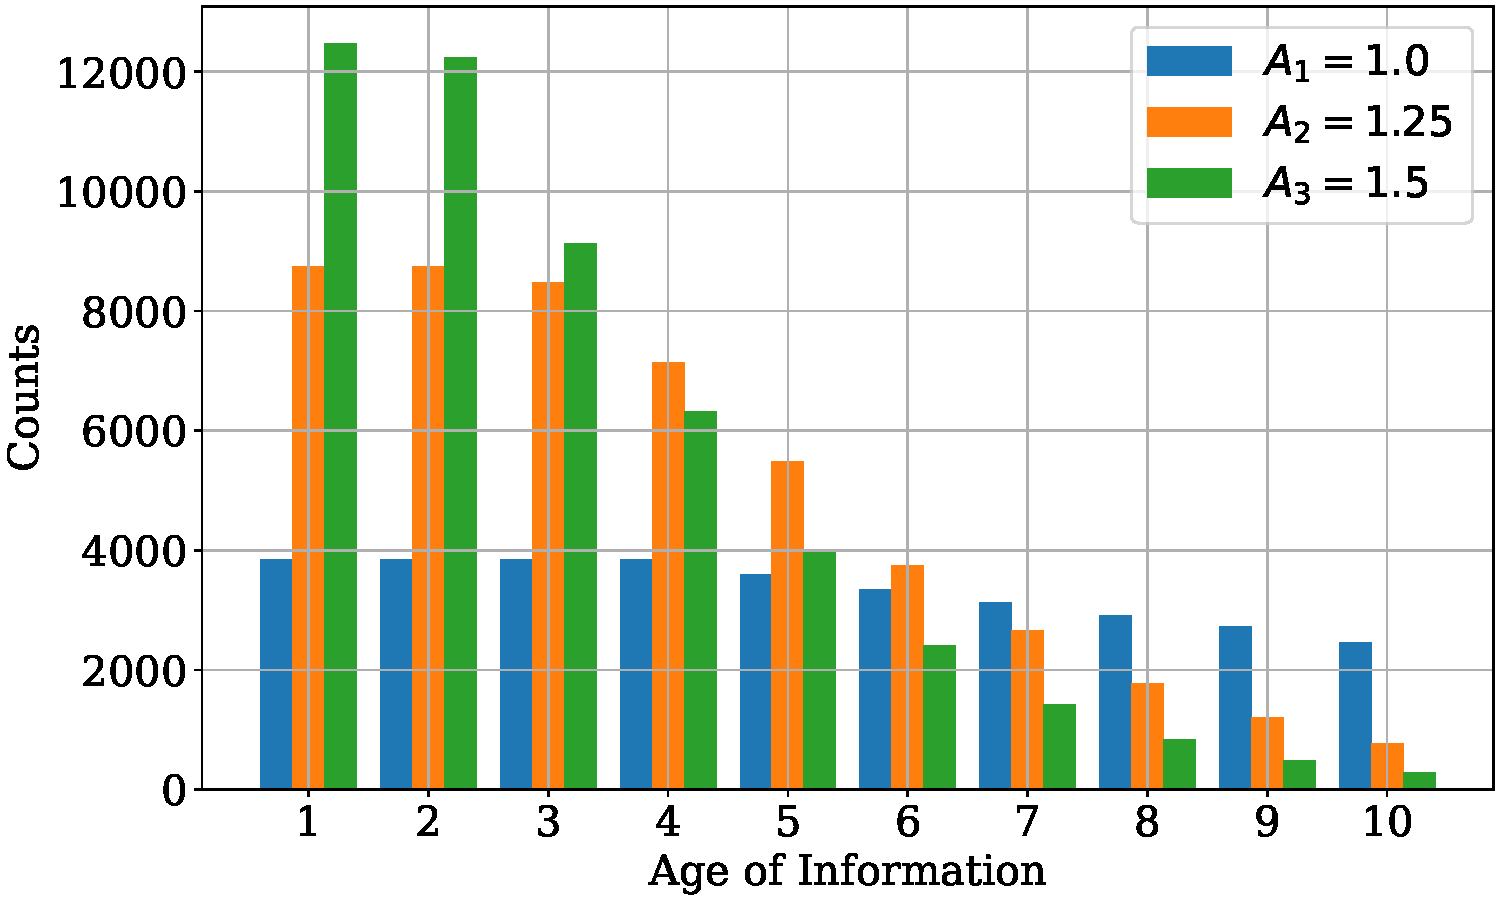
\includegraphics[width=\textwidth]{AoI_Histogram_N3_WC}
      \caption{Scenario 1 with GES}
  \end{subfigure}
  \begin{subfigure}[b]{0.49\textwidth}
      \centering
      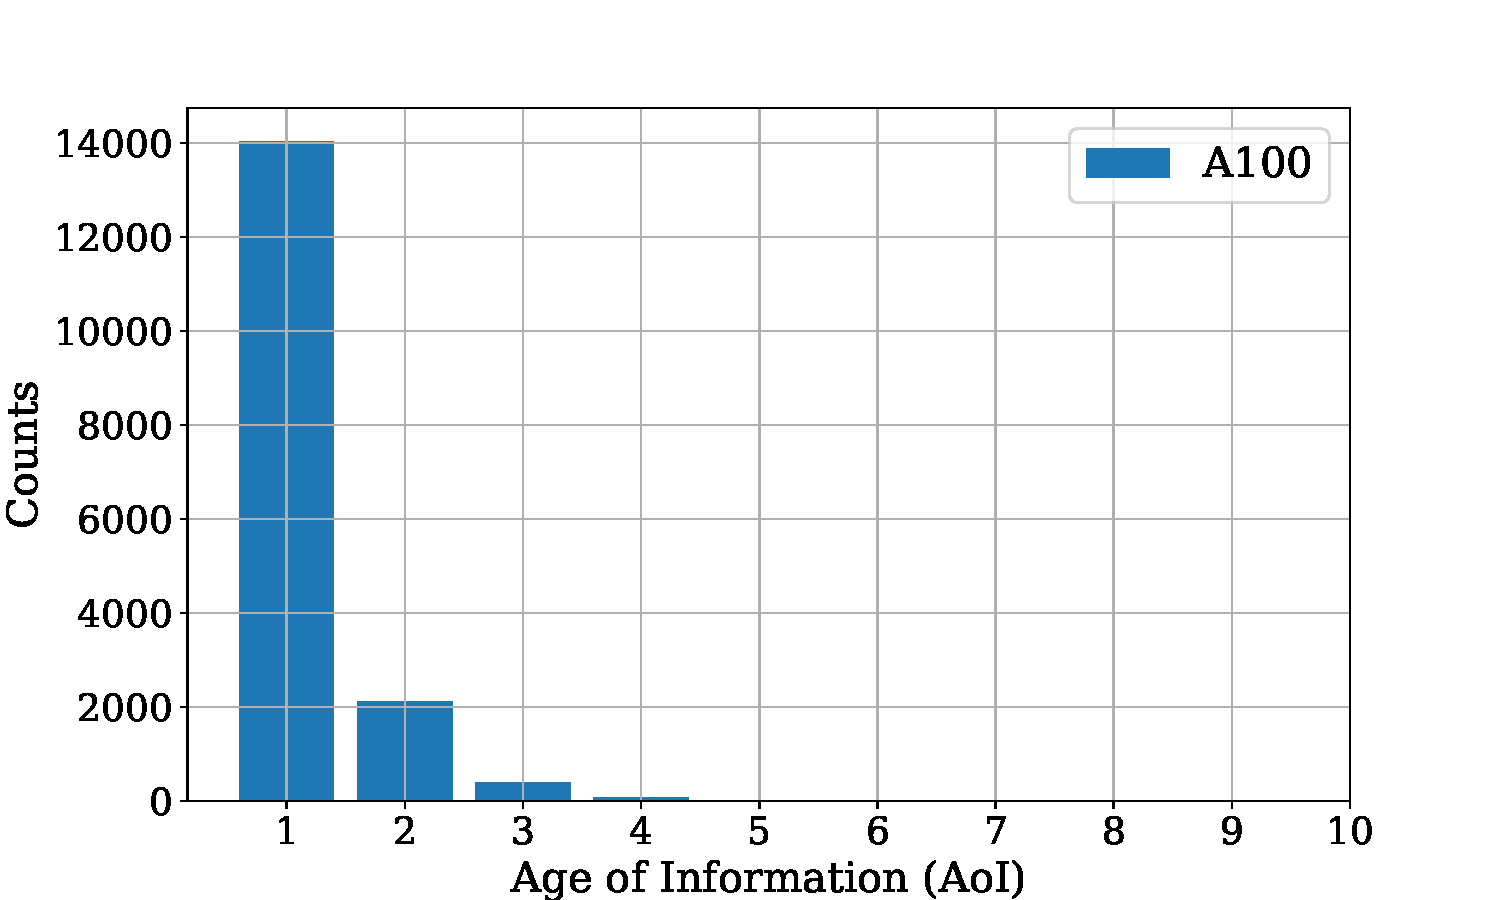
\includegraphics[width=\textwidth]{AoI_Histogram_A100}
      \caption{Scenario 1 with GES}
  \end{subfigure}
  \begin{subfigure}[b]{0.49\textwidth}
      \centering
      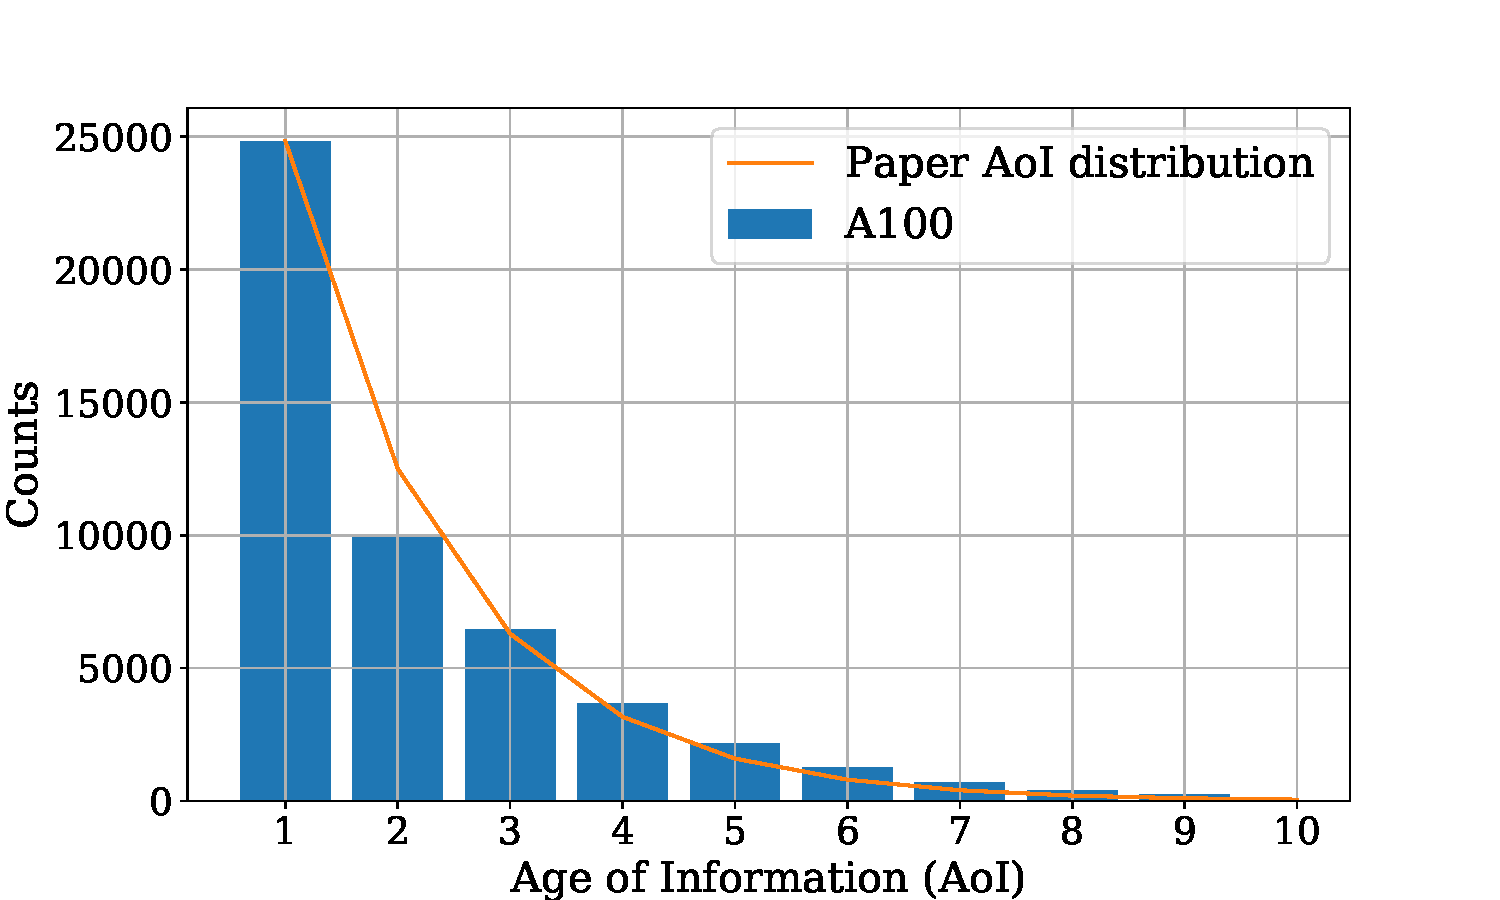
\includegraphics[width=\textwidth]{AoI_Histogram_A100_WC}
      \caption{Scenario 1 with GES}
  \end{subfigure}
     \caption[Test]{Test}
     \label{fig:AoIHist}
\end{figure}

\subsection{Complexity Analysis}
